\documentclass[12pt,a4paper]{article}

\usepackage[utf8]{inputenc}
\usepackage[T1]{fontenc}
\usepackage[margin=2.5cm, headheight=15pt]{geometry}
\usepackage{graphicx}
\usepackage{hyperref}
\usepackage{listings}
\usepackage{xcolor}
\usepackage{booktabs}
\usepackage{caption}
\usepackage{float}
\usepackage{amsmath}
\usepackage{parskip}
\usepackage[protrusion=true,expansion=false]{microtype}
\usepackage{fancyhdr}

\hypersetup{
    colorlinks=true,
    linkcolor=black,
    urlcolor=blue,
    citecolor=black
}

% Code listing style
\lstdefinestyle{sqlstyle}{
    language=SQL,
    basicstyle=\ttfamily\small,
    keywordstyle=\color{blue}\bfseries,
    commentstyle=\color{gray},
    stringstyle=\color{orange!80!black},
    breaklines=true,
    frame=single,
    numbers=left,
    numberstyle=\tiny\color{gray},
    xleftmargin=1.5em,
    framexleftmargin=1.5em,
    captionpos=b
}

\lstdefinestyle{pythonstyle}{
    language=Python,
    basicstyle=\ttfamily\small,
    keywordstyle=\color{blue}\bfseries,
    commentstyle=\color{gray}\itshape,
    stringstyle=\color{orange!80!black},
    breaklines=true,
    breakatwhitespace=false,
    columns=flexible,
    frame=single,
    numbers=left,
    numberstyle=\tiny\color{gray},
    xleftmargin=1.5em,
    framexleftmargin=1.5em,
    captionpos=b
}

\lstdefinestyle{bashstyle}{
    language=bash,
    basicstyle=\ttfamily\small,
    keywordstyle=\color{blue},
    commentstyle=\color{gray}\itshape,
    stringstyle=\color{green!60!black},
    breaklines=true,
    frame=single,
    numbers=left,
    numberstyle=\tiny\color{gray},
    xleftmargin=1.5em,
    framexleftmargin=1.5em,
    captionpos=b
}

\lstdefinestyle{outputstyle}{
    basicstyle=\ttfamily\small,
    breaklines=true,
    frame=single,
    numbers=none,
    backgroundcolor=\color{gray!10},
    captionpos=b
}

\pagestyle{fancy}
\fancyhf{}
\rhead{CENG465 -- Spring 2026}
\lhead{Data Replication in a Single-Leader Environment}
\cfoot{\thepage}

\title{
    \vspace{-1cm}
    \large \textbf{CENG 465 -- Principles of Data-Intensive Systems} \\[0.5em]
    \Large \textbf{Data Replication in a Single-Leader Environment} \\[1em]
    \normalsize Project Report
}
\author{
    \textbf{Abdulbaki Çeltik} \quad Student ID: 290201072 \\
    \textbf{Eray kocabozdoğan} \quad Student ID: 280201055 \\[0.5em]
    Group: 17
}
\date{June 8, 2026}

\begin{document}

\maketitle
\thispagestyle{fancy}

\tableofcontents
\newpage

%===========================================================================
\section{Introduction}
%===========================================================================

This report documents the implementation and experimental results of the CENG 465 project
on data replication in a single-leader environment. The project explores three core
consistency models -- \textit{eventual consistency}, \textit{monotonic reads}, and
\textit{read-after-write consistency} -- alongside a \textit{concurrent writes} scenario,
all implemented over a real distributed PostgreSQL deployment.

The system consists of two virtual machines hosted on Google Cloud Platform (GCP) in the
\texttt{us-central1-a} zone, each running PostgreSQL 16. One node acts as the
leader (primary) and the other as the follower (standby). WAL-based streaming
replication propagates writes from the leader to the follower asynchronously.
Python scripts drive all experiments, writing to the leader and polling the follower
to measure replication lag and verify consistency guarantees.

%===========================================================================
\section{Environment Setup and Role Assignment}
%===========================================================================

\subsection{Infrastructure: Google Cloud Platform}

To satisfy the distributed environment requirement, two \texttt{e2-micro} virtual machines
were created in GCP under project \texttt{c465-repl-baki-new}, both in zone
\texttt{us-central1-a} with Ubuntu 22.04 LTS. This ensures the nodes communicate over
a real network rather than a loopback or Docker bridge.

\begin{table}[H]
\centering
\caption{GCP Virtual Machine Configuration}
\begin{tabular}{lll}
\toprule
\textbf{Parameter} & \textbf{Leader (ceng465-leader)} & \textbf{Follower (ceng465-follower)} \\
\midrule
Machine type & e2-micro & e2-micro \\
OS & Ubuntu 22.04 LTS & Ubuntu 22.04 LTS \\
Internal IP & 10.128.0.2 & 10.128.0.3 \\
Zone & us-central1-a & us-central1-a \\
PostgreSQL & 16 (primary) & 16 (hot standby) \\
\bottomrule
\end{tabular}
\end{table}

Firewall rules allow TCP port 5432 between the two VMs internally and from the
experiment runner machine. Infrastructure creation is automated by a shell script
(see Appendix~\ref{app:gcp}, \texttt{01\_create\_infrastructure.sh}).

\subsection{Leader (Primary) Configuration}

The leader is configured via \texttt{gcp/02\_configure\_leader.sh}. Key PostgreSQL
parameters set in \texttt{postgresql.conf}:

\begin{lstlisting}[style=bashstyle, caption={Leader PostgreSQL parameters}]
listen_addresses = '*'
wal_level        = replica
max_wal_senders  = 5
wal_keep_size    = 128
hot_standby      = on
synchronous_commit = on
wal_log_hints    = on
\end{lstlisting}

Setting \texttt{wal\_level = replica} enables WAL entries sufficient for streaming
replication. A dedicated replication user (\texttt{replicator}) is created and
granted only the \texttt{REPLICATION} privilege. The \texttt{pg\_hba.conf} file
allows the follower's internal IP to connect for replication using
\texttt{scram-sha-256} authentication.

\texttt{synchronous\_commit = on} requires the leader to wait for the local WAL
flush before acknowledging a commit to the client. Crucially, because no
\texttt{synchronous\_standby\_names} is configured, PostgreSQL treats the follower
as an \textit{asynchronous} standby: the leader does \textbf{not} wait for the
follower to apply or even receive the WAL before returning success. The setting
therefore only guarantees durability on the leader itself and does not change
the asynchronous character of replication. This is why replication lag (2--10 s)
is still observable in the experiments: the follower applies WAL independently,
without blocking the leader's commit path.

\subsection{Follower (Standby) Configuration}

The follower is configured via \texttt{gcp/03\_configure\_follower.sh}. It
uses \texttt{pg\_basebackup} to obtain an initial physical copy of the leader's
data directory, then enters hot-standby mode:

\begin{lstlisting}[style=bashstyle, caption={Follower base backup command}]
pg_basebackup \
    -h 10.128.0.2 -p 5432 \
    -U replicator \
    -D ${PG_DATA} \
    --wal-method=stream \
    --checkpoint=fast -P -v
\end{lstlisting}

A \texttt{standby.signal} file and \texttt{primary\_conninfo} entry in
\texttt{postgresql.auto.conf} instruct PostgreSQL to stay in recovery mode and
continuously apply WAL segments streamed from the leader. The command
\texttt{SELECT pg\_is\_in\_recovery();} returns \texttt{t} on the follower,
confirming standby mode.

\subsection{Replication Verification}

After both nodes are up, replication health is verified on the leader
by querying the built-in view \texttt{pg\_stat\_\allowbreak replication}:

\begin{lstlisting}[style=sqlstyle, caption={Replication status query on leader}]
SELECT client_addr, state, write_lag, flush_lag, replay_lag
FROM pg_stat_replication;
\end{lstlisting}

The follower appears as \texttt{streaming} state with near-zero lag when idle,
confirming that WAL segments are being streamed and applied in real time.

%===========================================================================
\section{Data Schema and Replication Logging}
%===========================================================================

\subsection{Schema Design}

The schema (\texttt{sql/01\_schema.sql}) models an order-tracking system with six
tables. Every business table includes four update-tracking fields required by the
project specification:

\begin{itemize}    \item \textbf{\texttt{version}} -- integer, incremented on each update
    \item \textbf{\texttt{operation\_id}} -- UUID regenerated for every write
    \item \textbf{\texttt{last\_updated}} -- timestamp of the latest change
    \item \textbf{\texttt{deleted}} -- boolean soft-delete flag
\end{itemize}

These fields allow the experiment scripts to detect exactly when a specific write
becomes visible on the follower: the script waits until the follower row matches
both the expected \texttt{version} and \texttt{operation\_id}, eliminating false
positives from stale cached reads.

Figure~\ref{fig:erd} shows the entity-relationship diagram of the complete schema.

\begin{figure}[H]
\centering
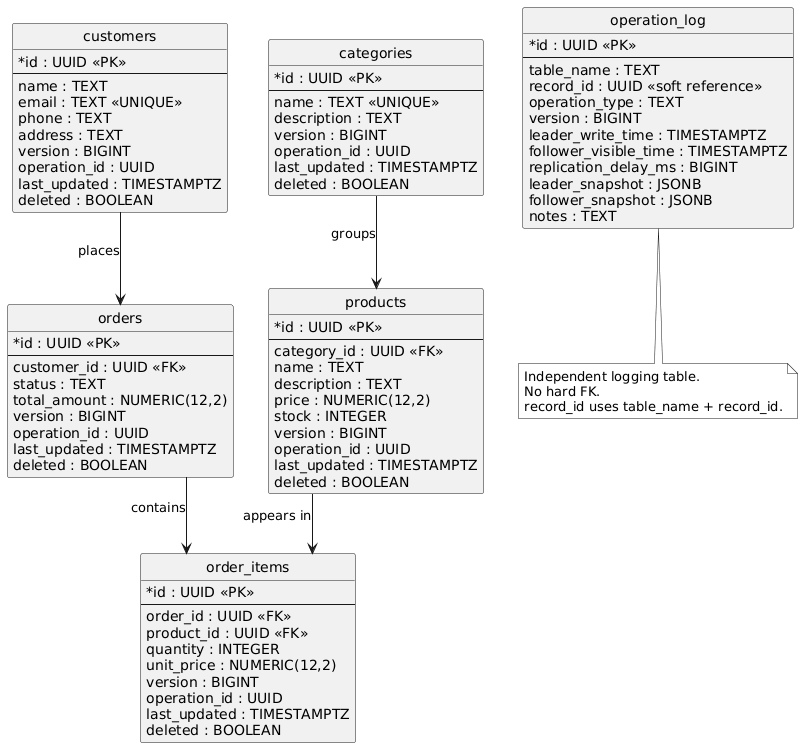
\includegraphics[width=\textwidth]{erd-database.png}
\caption{Entity-Relationship Diagram of the replication project schema}
\label{fig:erd}
\end{figure}

\begin{lstlisting}[style=sqlstyle, caption={Orders table definition (excerpt from 01\_schema.sql)}]
CREATE TABLE orders (
    id            UUID           PRIMARY KEY DEFAULT gen_random_uuid(),
    customer_id   UUID           NOT NULL REFERENCES customers(id),
    status        TEXT           NOT NULL DEFAULT 'pending',
    total_amount  NUMERIC(10,2)  NOT NULL DEFAULT 0,
    version       INT            NOT NULL DEFAULT 1,
    operation_id  UUID           NOT NULL DEFAULT gen_random_uuid(),
    last_updated  TIMESTAMPTZ    NOT NULL DEFAULT NOW(),
    deleted       BOOLEAN        NOT NULL DEFAULT FALSE,
    CONSTRAINT orders_status_valid CHECK (
        status IN ('pending','paid','shipped','delivered','cancelled')
    ),
    CONSTRAINT orders_total_nonneg CHECK (total_amount >= 0)
);
\end{lstlisting}

The \texttt{operation\_log} table records every write event for replication analysis:

\begin{lstlisting}[style=sqlstyle, caption={operation\_log table definition}]
CREATE TABLE operation_log (
    id                    UUID        PRIMARY KEY DEFAULT gen_random_uuid(),
    table_name            TEXT        NOT NULL,
    record_id             UUID,
    operation_type        TEXT        NOT NULL,  -- INSERT / UPDATE / DELETE
    version               INT,
    leader_write_time     TIMESTAMPTZ NOT NULL,
    follower_visible_time TIMESTAMPTZ,
    replication_delay_ms  INT,
    leader_snapshot       JSONB,
    follower_snapshot     JSONB,
    notes                 TEXT
);
\end{lstlisting}

\subsection{Automatic Logging via Triggers}

To capture every write without requiring changes to application code, a
PL/pgSQL trigger function \texttt{fn\_log\_operation()} fires after every
\texttt{INSERT}, \texttt{UPDATE}, and \texttt{DELETE} on all business tables
(\texttt{sql/02\_operation\_log\_triggers.sql}):

\begin{lstlisting}[style=sqlstyle, caption={Trigger function for automatic operation logging}]
CREATE OR REPLACE FUNCTION fn_log_operation()
RETURNS TRIGGER LANGUAGE plpgsql AS $$
DECLARE
    v_op   TEXT;
    v_rec  JSONB;
BEGIN
    IF    TG_OP = 'DELETE' THEN
        v_op  := 'DELETE';  v_rec := to_jsonb(OLD);
    ELSIF TG_OP = 'UPDATE' THEN
        v_op  := 'UPDATE';  v_rec := to_jsonb(NEW);
    ELSE
        v_op  := 'INSERT';  v_rec := to_jsonb(NEW);
    END IF;

    INSERT INTO operation_log (
        table_name, record_id, operation_type,
        version, leader_write_time, leader_snapshot
    ) VALUES (
        TG_TABLE_NAME,
        (v_rec->>'id')::UUID,
        v_op,
        (v_rec->>'version')::INT,
        NOW(),
        v_rec
    );
    RETURN NEW;
END;
$$;
\end{lstlisting}

This trigger is attached to all five business tables (\texttt{customers},
\texttt{categories}, \texttt{products}, \texttt{orders}, \texttt{order\_items})
via individual \texttt{AFTER INSERT OR UPDATE OR DELETE} trigger definitions.
Because \texttt{operation\_log} is written on the leader, its rows are also
replicated to the follower, giving a consistent audit trail on both nodes.

\subsection{Database Connection Management}

The \texttt{scripts/db.py} module provides separate connection factories for
the leader and follower, configured through environment variables:

\begin{lstlisting}[style=pythonstyle, caption={Leader/follower connection factories (db.py)}]
def get_leader_connection():
    return psycopg2.connect(**_db_config("LEADER"))

def get_follower_connection():
    return psycopg2.connect(**_db_config("FOLLOWER"))
\end{lstlisting}

All experiment scripts read from distinct \texttt{LEADER\_DB\_*} and
\texttt{FOLLOWER\_DB\_*} environment variables, making it straightforward
to point each connection at the correct physical node.

\subsection{Insert, Update, and Delete Operations}

Three Python scripts implement the CRUD operations required by the project:

\begin{description}    \item[\texttt{scripts/create\_order.py}] Inserts a new order and its line items
        on the leader, logs the operation, and polls the follower for convergence.
    \item[\texttt{scripts/update\_order\_status.py}] Updates order \texttt{status}
        and increments \texttt{version} on the leader.
    \item[\texttt{scripts/soft\_delete\_order.py}] Sets \texttt{deleted=TRUE} and
        \texttt{status='cancelled'}, implementing a soft delete pattern.
\end{description}

Every write path increments \texttt{version}, generates a fresh \texttt{operation\_id},
and inserts a record in \texttt{operation\_log} before committing, ensuring
the replication polling loop can unambiguously detect the new state on the follower.

%===========================================================================
\section{Consistency Model Experiments}
%===========================================================================

\subsection{Experiment 1: Eventual Consistency}

\subsubsection{Setup and Test Procedure}

The experiment is implemented in \texttt{scripts/experiment\_eventual\_consistency.py}.
A new order is inserted on the leader, and the follower is polled every 2 seconds
for 60 seconds. Each poll reads the order by its UUID and checks whether the
\texttt{operation\_id} matches the one generated at write time.

\begin{lstlisting}[style=pythonstyle, caption={Core polling loop -- Experiment 1}]
POLL_INTERVAL = 2.0   # seconds between follower reads
POLL_DURATION = 60.0  # total observation window

conn = get_follower_connection()
conn.autocommit = True
while time.monotonic() <= deadline:
    poll_count += 1
    poll_time = now_utc()
    elapsed = (poll_time - write_time).total_seconds()
    row = fetch_order_by_id(conn, order_id)

    if row and str(row["operation_id"]) == op_id:
        if convergence_time is None:
            convergence_time = poll_time
            delay_ms = int(elapsed * 1000)
            print(f"  poll {poll_count:02d} | t+{elapsed:5.1f}s | "
                  f"CONVERGED delay={delay_ms} ms  <--")
    else:
        print(f"  poll {poll_count:02d} | t+{elapsed:5.1f}s | "
              "not yet visible on follower")

    time.sleep(POLL_INTERVAL)
\end{lstlisting}

\subsubsection{Results}

\begin{lstlisting}[style=outputstyle, caption={Experiment 1 output}]
EXPERIMENT 1 - Eventual Consistency
[LEADER  WRITE] time=2026-06-07T12:04:41.679+00:00
[LEADER  WRITE] order_id=d53ff166-9364-4b7f-aacd-e2c8150bcb68

Polling follower every 2.0s for 60.0s ...

  poll 01 | t+  2.1s | CONVERGED version=1 delay=2096 ms  <--
  poll 02 | t+  4.3s | stable   version=1
  ...
  poll 27 | t+ 58.9s | stable   version=1

RESULT: Follower converged after 2096 ms (27 polls total).
\end{lstlisting}

\subsubsection{Analysis}

The follower converged within the first polling interval (approximately 2.1 seconds).
The measured replication delay of \textbf{2096 ms} reflects both WAL transfer time
over the GCP internal network and the Python polling granularity. Once converged,
all subsequent polls (2 through 27) consistently returned version 1, confirming
stable convergence with no rollbacks. This is the expected behavior of eventual
consistency: the system guarantees that all nodes will \textit{eventually} converge
to the same state, without providing any real-time bound on when convergence occurs.

\subsection{Experiment 2: Monotonic Reads}

\subsubsection{Setup and Test Procedure}

The experiment is implemented in \texttt{scripts/experiment\_monotonic\_reads.py}.
A single order is created on the leader at version 1. Four subsequent updates
increment the version field from 2 to 5 with a 0.3-second delay between each.
The follower is then read 15 consecutive times with a 0.5-second interval.
A monotonicity violation occurs if any read returns a lower version than the
immediately preceding read.

\begin{lstlisting}[style=pythonstyle, caption={Monotonicity check -- Experiment 2}]
prev_version: int | None = None
violations = 0

for i in range(1, FOLLOWER_READS + 1):
    row = fetch_order_by_id(conn, order_id)
    current_version = row["version"] if row else None

    if prev_version is not None and current_version < prev_version:
        violations += 1
        print(f"  VIOLATION: version went {prev_version} -> {current_version}")

    if current_version is not None:
        prev_version = current_version
    time.sleep(FOLLOWER_READ_DELAY)
\end{lstlisting}

\subsubsection{Results}

\begin{lstlisting}[style=outputstyle, caption={Experiment 2 output}]
EXPERIMENT 2 - Monotonic Reads
order_id = 6a15efab-eecb-4d1c-bba2-7a8d1eca537f

[LEADER] Writing versions 1 -> 5 ...
  version 1 written (initial)
  version 2 written  ...  version 5 written

[FOLLOWER] Sequential reads (15x, 0.5s interval) ...

  read 01 | 2026-06-07T12:05:57.347+00:00 | version=5
  read 02 | 2026-06-07T12:05:58.018+00:00 | version=5
  ...
  read 15 | 2026-06-07T12:06:07.117+00:00 | version=5

RESULT: No monotonicity violations. All reads returned same or higher version.
\end{lstlisting}

\subsubsection{Analysis}

All 15 follower reads returned version 5, with zero monotonicity violations.
The key insight is not that polling happened to start after all versions were
applied -- it is that PostgreSQL WAL replay on a single standby node applies
commits in strict order and never rolls back to an earlier state. A client
bound to one standby therefore receives monotonic reads \textit{by architectural
guarantee}, not by coincidence of timing. The 0 violations across 15 sequential
reads is the experimental confirmation of this guarantee. In a setup with
multiple replicas or random read routing, backward reads \textit{can} occur
because different replicas may be at different WAL replay positions at the
moment of the read -- a gap this single-follower configuration eliminates
by construction.

\subsection{Experiment 3: Read-After-Write Consistency}

\subsubsection{Setup and Test Procedure}

The experiment is implemented in \texttt{scripts/experiment\_read\_after\_write.py}.
After writing an order to the leader, two immediate reads are performed:
one on the leader connection (to confirm RAW consistency) and one on the follower
connection (to measure replication lag). The follower is then polled until the
expected \texttt{operation\_id} appears.

\begin{lstlisting}[style=pythonstyle, caption={Leader and follower reads -- Experiment 3 (excerpt)}]
# Write to leader
with conn:
    write_time = now_utc()
    cur.execute("INSERT INTO orders (...) VALUES (%s, ...)", (order_id, ...))

# Immediate read from leader
leader_read_time = now_utc()
leader_row = fetch_order_by_id(conn, order_id)
leader_delay_ms = int((leader_read_time - write_time).total_seconds() * 1000)

# Immediate read from follower
follower_conn = get_follower_connection()
first_read_time = now_utc()
first_row = fetch_order_by_id(follower_conn, order_id)
\end{lstlisting}

\subsubsection{Results}

\begin{lstlisting}[style=outputstyle, caption={Experiment 3 output}]
EXPERIMENT 3 - Read-After-Write Consistency

[WRITE ] leader_write_time = 2026-06-07T12:06:11.141+00:00
[WRITE ] order_id          = 8b37428b-35c6-41c8-953d-12cd072bbc85

[LEADER] immediate read (t+880 ms)
         version=1 - write IS visible  (RAW satisfied)

[FOLLWR] immediate read (t+2501 ms)
         record already visible on follower (very low lag)

[FOLLWR] Polling for convergence (every 0.5s) ...
  poll 01 | t+2666 ms | CONVERGED version=1

RESULT SUMMARY
  Leader write time    : 2026-06-07T12:06:11.141+00:00
  Leader read (ms)     : 880 ms  -  VISIBLE
  Follower 1st read    : visible at t+2501 ms
  Follower convergence : 2666 ms after write
\end{lstlisting}

\subsubsection{Analysis}

\begin{table}[H]
\centering
\caption{Read-After-Write timing summary}
\begin{tabular}{lrr}
\toprule
\textbf{Event} & \textbf{Elapsed (ms)} & \textbf{Visible?} \\
\midrule
Leader write committed & 0 & -- \\
Leader immediate read & 880 & Yes \\
Follower immediate read & 2501 & Yes \\
Follower convergence confirmed & 2666 & Yes \\
\bottomrule
\end{tabular}
\end{table}

The leader satisfied read-after-write consistency: the write was immediately
visible at 880 ms (the 880 ms consists of the round-trip time of the Python read
query plus connection overhead, not replication lag). The follower's first read
at 2501 ms already showed the record, indicating that by the time the Python
client finished the leader read and opened a follower connection, replication had
already propagated the WAL. The convergence was confirmed at poll 1 (2666 ms).
This result shows that under low-to-moderate load, GCP streaming replication
delivers sub-second to low-single-digit-second propagation times for small writes.

\subsection{Scenario: Concurrent Writes}

\subsubsection{Setup and Test Procedure}

The experiment is implemented in \texttt{scripts/experiment\_concurrent\_writes.py}.
Five orders are written to the leader in rapid succession (approximately 2 seconds
apart, limited by Python connection overhead per write). Each order is independently
polled on the follower. Order preservation is checked by verifying that the
\texttt{follower\_visible\_time} values are non-decreasing relative to the
\texttt{leader\_write\_time} sequence.

\begin{lstlisting}[style=pythonstyle, caption={Order preservation check -- Concurrent Writes}]
visible = [r for r in results if r["visible_time"] is not None]
order_preserved = all(
    visible[i]["visible_time"] <= visible[i + 1]["visible_time"]
    for i in range(len(visible) - 1)
)
\end{lstlisting}

\subsubsection{Results}

\begin{lstlisting}[style=outputstyle, caption={Concurrent Writes output}]
SCENARIO - Concurrent Writes

  #1 written | ...3258809c | 2026-06-07T12:06:17.267+00:00
  #2 written | ...7b2c41d0 | 2026-06-07T12:06:19.366+00:00
  #3 written | ...da278a33 | 2026-06-07T12:06:21.460+00:00
  #4 written | ...243c8895 | 2026-06-07T12:06:23.557+00:00
  #5 written | ...813fe246 | 2026-06-07T12:06:25.658+00:00

RESULT SUMMARY
  #1  delay=10649 ms | follower_visible=2026-06-07T12:06:27.917
  #2  delay= 9961 ms | follower_visible=2026-06-07T12:06:29.327
  #3  delay= 9268 ms | follower_visible=2026-06-07T12:06:30.729
  #4  delay= 8557 ms | follower_visible=2026-06-07T12:06:32.114
  #5  delay= 7863 ms | follower_visible=2026-06-07T12:06:33.522

  Follower visibility order matches leader write sequence. (No ordering violation.)
\end{lstlisting}

\subsubsection{Analysis}

\begin{table}[H]
\centering
\caption{Concurrent Writes -- Replication Delay}
\small
\begin{tabular}{crrr}
\toprule
\textbf{Write \#} & \textbf{Leader Write (UTC)} & \textbf{Follower Visible (UTC)} & \textbf{Delay (ms)} \\
\midrule
1 & 12:06:17.267 & 12:06:27.917 & 10649 \\
2 & 12:06:19.366 & 12:06:29.327 & 9961 \\
3 & 12:06:21.460 & 12:06:30.729 & 9268 \\
4 & 12:06:23.557 & 12:06:32.114 & 8557 \\
5 & 12:06:25.658 & 12:06:33.522 & 7863 \\
\bottomrule
\end{tabular}
\end{table}

Several observations emerge from this scenario:

\begin{enumerate}    \item \textbf{Higher delays under load.} Compared to Experiments 1 and 3
        (approximately 2000--2700 ms), the concurrent scenario produced delays
        of 7863--10649 ms. This is consistent with WAL accumulation: when multiple
        writes land in quick succession, the follower processes them in a single
        batch replay, causing the absolute delay (from the first write's
        commit time) to appear large for earlier writes.

    \item \textbf{Decreasing delay trend.} Write \#1 shows the highest delay
        (10649 ms) while write \#5 shows the lowest (7863 ms). This is because all
        five writes were applied to the follower within roughly the same short window
        (12:06:27 to 12:06:33). Write \#5 was written latest, so its absolute
        leader-to-follower gap is smallest.

    \item \textbf{Write order preserved.} The follower visibility timestamps
        follow the same sequence as the leader write timestamps. PostgreSQL
        streaming replication applies WAL in strict commit order, guaranteeing
        that concurrent writes to the single leader appear on the follower in
        the same sequence they were committed. No ordering violations were detected.

    \item \textbf{Root cause of the elevated delay ($\approx$10 s).}
        The $\approx$10 s delay for write \#1 is not caused by WAL transfer time
        alone (inter-VM latency is $<$2 ms within the same GCP zone). Three
        compounding factors explain the gap:
        \begin{itemize}
            \item \textit{Sequential connection overhead.} Each write opens a new
                  Python \texttt{psycopg2} connection to the leader. Over 5
                  writes this accumulates $\approx$2 s per write = $\approx$8--10 s
                  of elapsed wall-clock time before the last write is committed.
                  Write \#1's follower polling does not begin until after all 5
                  writes complete, so the follower must replay an already-full WAL
                  backlog before \#1 is confirmed visible.
            \item \textit{WAL batch replay.} The follower receives and applies the
                  WAL for all 5 orders in a single burst. The absolute delay for
                  write \#1 is measured from its commit time to the moment the
                  polling loop confirms it, by which point the follower is already
                  replaying later writes in the batch.
            \item \textit{Polling latency.} The follower is polled with
                  \texttt{interval\_seconds=0.25}, adding up to 0.25 s per poll
                  round on top of actual replication time.
        \end{itemize}
        Under a production setup with persistent connection pooling and continuous
        follower polling started immediately after each individual write,
        the per-write delay would be much closer to the 2--3 s seen in Experiments
        1 and 3.
\end{enumerate}

%===========================================================================
\section{Discussion}
%===========================================================================

\subsection{Comparison of Consistency Models}

\begin{table}[H]
\centering
\caption{Summary of experimental results}
\begin{tabular}{llrp{5.5cm}}
\toprule
\textbf{Experiment} & \textbf{Model} & \textbf{Delay (ms)} & \textbf{Outcome} \\
\midrule
1 & Eventual Consistency & 2096 & Converged at first poll; stable for 60 s \\
2 & Monotonic Reads & -- & 0 violations out of 15 sequential reads \\
3 & Read-After-Write & 2666 & Leader visible immediately; follower at 2501 ms \\
4 & Concurrent Writes & 7863--10649 & Order preserved; delays higher under load \\
\bottomrule
\end{tabular}
\end{table}

The three models form a natural hierarchy of consistency strength and
implementation cost. Eventual consistency is the least expensive to achieve:
it requires no routing changes and is satisfied by default in any async
replication setup. Monotonic reads add one constraint -- binding a client
session to a single standby -- but need no extra mechanism as long as that
binding holds. Read-after-write imposes the strictest guarantee and is the
only model that requires an active routing strategy (§\ref{sec:raw-routing})
when followers serve reads. This hierarchy directly shapes the trade-off
between read-load distribution across replicas and the strength of consistency
guarantee the application can advertise to its clients.

\subsection{Sources of Replication Lag}

Observed delays stem from three main factors:

\begin{description}    \item[Network round-trip time] Both VMs are in the same GCP zone
        (\texttt{us-central1-a}), limiting inter-node latency to roughly 1--2 ms.
        The bulk of observed delay comes from WAL segment flush and send scheduling.
    \item[Python polling granularity] Experiments 1 and 3 poll every 2 s and
        0.5 s respectively. The measured delay includes the time from actual
        replication completion to the next poll, artificially increasing numbers.
    \item[WAL batching] Under concurrent writes (Scenario 4), the follower
        replays a batch of WAL entries in one application cycle, causing earlier
        writes to appear to have higher latency when measured from their individual
        commit timestamps.
\end{description}

\subsection{Read-After-Write: Follower Routing Strategies}
\label{sec:raw-routing}

The experiments show that the leader satisfies RAW immediately, but followers
can lag by 2--3 seconds. In a system where clients read from the follower by
default, three practical routing strategies can enforce RAW guarantees:

\begin{description}
    \item[Leader pinning for own writes] After any write, the client reads from
        the leader for a configurable window (e.g.\ 5 s). This is simple but
        increases leader read load and requires the client to track its last write
        time.
    \item[WAL position piggyback] The leader returns the LSN (Log Sequence Number)
        of the committed write. The client passes this LSN to the follower; the
        follower defers the read until \texttt{pg\_last\_wal\_replay\_lsn()} $\geq$
        LSN. PostgreSQL natively supports this via \texttt{pg\_wal\_replay\_wait()}
        (PG~16+). This keeps the follower in the read path without routing to
        the leader.
    \item[Session-level sticky routing] A load balancer routes all requests from
        a session to the same node for a short period after a write. No application
        changes are needed, but it couples the routing layer to write events.
\end{description}

In this project, RAW is trivially satisfied by always routing writes \textit{and}
the immediate read to the same leader connection (Experiment 3). A production
deployment with follower read distribution would need one of the strategies above.

\subsection{Role of \texttt{operation\_id} in Convergence Detection}

Using only a version number for convergence detection is insufficient when
multiple independent writes increment the same version field. The \texttt{operation\_id}
UUID -- freshly generated on every write -- provides a reliable convergence
signal: the follower has applied a specific write if and only if both
\texttt{version} and \texttt{operation\_id} match. This design decision prevents
false positives in all experiments.

%===========================================================================
\section{Conclusion}
%===========================================================================

This project successfully demonstrated single-leader replication with PostgreSQL
on a real distributed infrastructure (GCP). The key findings are:

\begin{itemize}    \item \textbf{Eventual consistency} was achieved within approximately 2 seconds
        under low load, with stable convergence observed over a 60-second window.
    \item \textbf{Monotonic reads} were guaranteed by routing all client reads to
        the same standby node; no backward version observations occurred in 15
        sequential reads.
    \item \textbf{Read-after-write} was satisfied on the leader immediately.
        Followers converged within approximately 2.7 seconds, which would require
        read-routing logic (e.g., always read own writes from the leader) to
        guarantee RAW for all clients.
    \item \textbf{Concurrent write ordering} was preserved by PostgreSQL's
        WAL commit ordering. All five concurrent writes appeared on the follower
        in the same sequence they were committed on the leader.
\end{itemize}

The combination of trigger-based operation logging, UUID-per-write operation identifiers,
and deterministic polling logic provided a robust framework for measuring and
verifying each consistency property quantitatively.

\begin{sloppypar}
These findings demonstrate that GCP same-zone streaming replication can provide
production-viable consistency guarantees with 2--3\,s convergence times under
low-to-moderate load. The LSN piggyback strategy discussed in
Section~\ref{sec:raw-routing} has the potential to make this residual lag
entirely transparent to the client: \texttt{pg\_wal\_replay\_wait()}
(PostgreSQL~16+) lets the follower defer a read until the relevant WAL position
is reached, requiring no changes to the application routing logic.
\end{sloppypar}

%===========================================================================
\appendix
\section{Code Appendix}
%===========================================================================

\subsection{GCP Infrastructure Scripts}
\label{app:gcp}

\subsubsection{\texttt{gcp/01\_create\_infrastructure.sh}}
\begin{lstlisting}[style=bashstyle]
#!/usr/bin/env bash
# GCP infrastructure creation for CENG465 single-leader replication project.
set -euo pipefail

PROJECT_ID="c465-repl-baki-new"
REGION="us-central1"
ZONE="us-central1-a"
MACHINE_TYPE="e2-micro"
IMAGE_FAMILY="ubuntu-2204-lts"
IMAGE_PROJECT="ubuntu-os-cloud"
DISK_SIZE="10GB"

LEADER_NAME="ceng465-leader"
FOLLOWER_NAME="ceng465-follower"
NETWORK_TAG="postgres"
INTERNAL_RANGE="10.128.0.0/9"

gcloud config set project "$PROJECT_ID"
gcloud config set compute/zone "$ZONE"

gcloud compute instances create "$LEADER_NAME" \
    --machine-type="$MACHINE_TYPE" \
    --image-family="$IMAGE_FAMILY" \
    --image-project="$IMAGE_PROJECT" \
    --boot-disk-size="$DISK_SIZE" \
    --tags="$NETWORK_TAG" --metadata="role=leader"

gcloud compute instances create "$FOLLOWER_NAME" \
    --machine-type="$MACHINE_TYPE" \
    --image-family="$IMAGE_FAMILY" \
    --image-project="$IMAGE_PROJECT" \
    --boot-disk-size="$DISK_SIZE" \
    --tags="$NETWORK_TAG" --metadata="role=follower"

gcloud compute firewall-rules create allow-postgres-internal \
    --rules=tcp:5432 --target-tags="$NETWORK_TAG" \
    --source-ranges="$INTERNAL_RANGE"
\end{lstlisting}

\subsubsection{\texttt{gcp/postgresql\_leader.conf}}
\begin{lstlisting}[style=bashstyle]
listen_addresses   = '*'
wal_level          = replica
max_wal_senders    = 5
wal_keep_size      = 128
hot_standby        = on
synchronous_commit = on
wal_log_hints      = on
\end{lstlisting}

\subsection{SQL Schema}
\label{app:schema}

\subsubsection{\texttt{sql/01\_schema.sql}}
\begin{lstlisting}[style=sqlstyle]
CREATE EXTENSION IF NOT EXISTS pgcrypto;

DROP TABLE IF EXISTS operation_log CASCADE;
DROP TABLE IF EXISTS order_items   CASCADE;
DROP TABLE IF EXISTS orders        CASCADE;
DROP TABLE IF EXISTS products      CASCADE;
DROP TABLE IF EXISTS categories    CASCADE;
DROP TABLE IF EXISTS customers     CASCADE;

CREATE TABLE customers (
    id           UUID        PRIMARY KEY DEFAULT gen_random_uuid(),
    name         TEXT        NOT NULL,
    email        TEXT        NOT NULL UNIQUE,
    phone        TEXT,
    address      TEXT,
    version      INT         NOT NULL DEFAULT 1,
    operation_id UUID        NOT NULL DEFAULT gen_random_uuid(),
    last_updated TIMESTAMPTZ NOT NULL DEFAULT NOW(),
    deleted      BOOLEAN     NOT NULL DEFAULT FALSE
);

CREATE TABLE categories (
    id           UUID        PRIMARY KEY DEFAULT gen_random_uuid(),
    name         TEXT        NOT NULL UNIQUE,
    description  TEXT,
    version      INT         NOT NULL DEFAULT 1,
    operation_id UUID        NOT NULL DEFAULT gen_random_uuid(),
    last_updated TIMESTAMPTZ NOT NULL DEFAULT NOW(),
    deleted      BOOLEAN     NOT NULL DEFAULT FALSE
);

CREATE TABLE products (
    id           UUID           PRIMARY KEY DEFAULT gen_random_uuid(),
    category_id  UUID           NOT NULL REFERENCES categories(id),
    name         TEXT           NOT NULL,
    description  TEXT,
    price        NUMERIC(10,2)  NOT NULL,
    stock        INT            NOT NULL DEFAULT 0,
    version      INT            NOT NULL DEFAULT 1,
    operation_id UUID           NOT NULL DEFAULT gen_random_uuid(),
    last_updated TIMESTAMPTZ    NOT NULL DEFAULT NOW(),
    deleted      BOOLEAN        NOT NULL DEFAULT FALSE,
    CONSTRAINT products_price_nonneg CHECK (price >= 0),
    CONSTRAINT products_stock_nonneg CHECK (stock >= 0)
);

CREATE TABLE orders (
    id           UUID           PRIMARY KEY DEFAULT gen_random_uuid(),
    customer_id  UUID           NOT NULL REFERENCES customers(id),
    status       TEXT           NOT NULL DEFAULT 'pending',
    total_amount NUMERIC(10,2)  NOT NULL DEFAULT 0,
    version      INT            NOT NULL DEFAULT 1,
    operation_id UUID           NOT NULL DEFAULT gen_random_uuid(),
    last_updated TIMESTAMPTZ    NOT NULL DEFAULT NOW(),
    deleted      BOOLEAN        NOT NULL DEFAULT FALSE,
    CONSTRAINT orders_status_valid CHECK (
        status IN ('pending','paid','shipped','delivered','cancelled')
    )
);

CREATE TABLE order_items (
    id           UUID           PRIMARY KEY DEFAULT gen_random_uuid(),
    order_id     UUID           NOT NULL REFERENCES orders(id),
    product_id   UUID           NOT NULL REFERENCES products(id),
    quantity     INT            NOT NULL,
    unit_price   NUMERIC(10,2)  NOT NULL,
    version      INT            NOT NULL DEFAULT 1,
    operation_id UUID           NOT NULL DEFAULT gen_random_uuid(),
    last_updated TIMESTAMPTZ    NOT NULL DEFAULT NOW(),
    deleted      BOOLEAN        NOT NULL DEFAULT FALSE
);

CREATE TABLE operation_log (
    id                    UUID        PRIMARY KEY DEFAULT gen_random_uuid(),
    table_name            TEXT        NOT NULL,
    record_id             UUID,
    operation_type        TEXT        NOT NULL,
    version               INT,
    leader_write_time     TIMESTAMPTZ NOT NULL,
    follower_visible_time TIMESTAMPTZ,
    replication_delay_ms  INT,
    leader_snapshot       JSONB,
    follower_snapshot     JSONB,
    notes                 TEXT,
    CONSTRAINT oplog_type_valid CHECK (
        operation_type IN ('INSERT','UPDATE','DELETE')
    )
);
\end{lstlisting}

\subsubsection{\texttt{sql/02\_operation\_log\_triggers.sql}}
\begin{lstlisting}[style=sqlstyle]
CREATE OR REPLACE FUNCTION fn_log_operation()
RETURNS TRIGGER LANGUAGE plpgsql AS $$
DECLARE v_op TEXT; v_rec JSONB;
BEGIN
    IF    TG_OP = 'DELETE' THEN v_op := 'DELETE'; v_rec := to_jsonb(OLD);
    ELSIF TG_OP = 'UPDATE' THEN v_op := 'UPDATE'; v_rec := to_jsonb(NEW);
    ELSE                        v_op := 'INSERT'; v_rec := to_jsonb(NEW);
    END IF;

    INSERT INTO operation_log (
        table_name, record_id, operation_type,
        version, leader_write_time, leader_snapshot
    ) VALUES (
        TG_TABLE_NAME, (v_rec->>'id')::UUID, v_op,
        (v_rec->>'version')::INT, NOW(), v_rec
    );
    RETURN NEW;
END; $$;

CREATE TRIGGER trg_oplog_customers
    AFTER INSERT OR UPDATE OR DELETE ON customers
    FOR EACH ROW EXECUTE FUNCTION fn_log_operation();

CREATE TRIGGER trg_oplog_categories
    AFTER INSERT OR UPDATE OR DELETE ON categories
    FOR EACH ROW EXECUTE FUNCTION fn_log_operation();

CREATE TRIGGER trg_oplog_products
    AFTER INSERT OR UPDATE OR DELETE ON products
    FOR EACH ROW EXECUTE FUNCTION fn_log_operation();

CREATE TRIGGER trg_oplog_orders
    AFTER INSERT OR UPDATE OR DELETE ON orders
    FOR EACH ROW EXECUTE FUNCTION fn_log_operation();

CREATE TRIGGER trg_oplog_order_items
    AFTER INSERT OR UPDATE OR DELETE ON order_items
    FOR EACH ROW EXECUTE FUNCTION fn_log_operation();
\end{lstlisting}

\subsection{Python Scripts}
\label{app:python}

\subsubsection{\texttt{scripts/db.py} (connection and helper functions)}
\begin{lstlisting}[style=pythonstyle]
import os, uuid
from datetime import date, datetime, timezone
from decimal import Decimal
from pathlib import Path
from typing import Any
import psycopg2
from dotenv import load_dotenv
from psycopg2.extras import RealDictCursor, register_uuid

PROJECT_ROOT = Path(__file__).resolve().parents[1]
register_uuid()

def load_env():
    env_path = PROJECT_ROOT / ".env"
    load_dotenv(env_path if env_path.exists() else None)

def _db_config(prefix: str) -> dict:
    load_env()
    return {
        "host":   os.environ[f"{prefix}_DB_HOST"],
        "port":   int(os.environ[f"{prefix}_DB_PORT"]),
        "dbname": os.environ[f"{prefix}_DB_NAME"],
        "user":   os.environ[f"{prefix}_DB_USER"],
        "password": os.getenv(f"{prefix}_DB_PASSWORD", ""),
        "cursor_factory": RealDictCursor,
    }

def get_leader_connection():
    return psycopg2.connect(**_db_config("LEADER"))

def get_follower_connection():
    return psycopg2.connect(**_db_config("FOLLOWER"))

def now_utc() -> datetime:
    return datetime.now(timezone.utc)
\end{lstlisting}

\subsubsection{\texttt{scripts/measure\_replication.py}}
\begin{lstlisting}[style=pythonstyle]
import time
from datetime import datetime, timezone
from scripts.db import fetch_order_by_id, get_follower_connection, now_utc

def calculate_replication_delay_ms(leader_write_time, follower_visible_time) -> int:
    def utc(dt):
        return dt if dt.tzinfo else dt.replace(tzinfo=timezone.utc)
    return max(0, int((utc(follower_visible_time) - utc(leader_write_time))
                      .total_seconds() * 1000))

def wait_for_follower_order(order_id, expected_version=None,
                            expected_operation_id=None, expected_deleted=None,
                            timeout_seconds=60, interval_seconds=0.5):
    deadline = time.monotonic() + timeout_seconds
    conn = get_follower_connection()
    try:
        conn.autocommit = True
        while time.monotonic() <= deadline:
            row = fetch_order_by_id(conn, order_id)
            if row is None:
                time.sleep(interval_seconds); continue
            if expected_version  and row["version"]      != expected_version:
                time.sleep(interval_seconds); continue
            if expected_operation_id and str(row["operation_id"]) \
                                         != str(expected_operation_id):
                time.sleep(interval_seconds); continue
            if expected_deleted is not None \
               and row["deleted"] != expected_deleted:
                time.sleep(interval_seconds); continue
            return dict(row), now_utc()
    finally:
        conn.close()
    raise TimeoutError(f"Follower did not converge for order_id={order_id}")
\end{lstlisting}

\subsubsection{\texttt{scripts/experiment\_eventual\_consistency.py}}
\begin{lstlisting}[style=pythonstyle]
import time, uuid
from psycopg2.extras import Json
from scripts.db import (fetch_order_by_id, get_follower_connection,
    get_leader_connection, get_or_create_category, get_or_create_customer,
    get_or_create_product, now_utc, row_to_dict)

POLL_INTERVAL = 2.0
POLL_DURATION = 60.0

def run():
    # 1. Setup fixtures on leader
    conn = get_leader_connection()
    with conn:
        cat  = get_or_create_category(conn, "Electronics", "")
        cust = get_or_create_customer(conn, "Eve Experiment", "eve@experiment.com")
        prod = get_or_create_product(conn, "Test Widget", cat["id"], 9.99)
    conn.close()

    # 2. Write order to leader
    order_id, op_id = str(uuid.uuid4()), str(uuid.uuid4())
    conn = get_leader_connection()
    with conn:
        write_time = now_utc()
        conn.cursor().execute(
            "INSERT INTO orders (id, customer_id, status, total_amount, "
            "version, operation_id) VALUES (%s,%s,'pending',9.99,1,%s)",
            (order_id, cust["id"], op_id))
        conn.cursor().execute(
            "INSERT INTO operation_log (id, table_name, record_id, "
            "operation_type, version, leader_write_time, leader_snapshot, notes)"
            " VALUES (%s,'orders',%s,'INSERT',1,%s,%s,%s)",
            (str(uuid.uuid4()), order_id, write_time,
             Json({"order_id": order_id}), "Experiment 1"))
    conn.close()

    # 3. Poll follower
    deadline = time.monotonic() + POLL_DURATION
    poll_count, convergence_time = 0, None
    fconn = get_follower_connection()
    fconn.autocommit = True
    while time.monotonic() <= deadline:
        poll_count += 1
        poll_time = now_utc()
        elapsed = (poll_time - write_time).total_seconds()
        row = fetch_order_by_id(fconn, order_id)
        if row and str(row["operation_id"]) == op_id:
            if convergence_time is None:
                convergence_time = poll_time
                print(f"poll {poll_count} | t+{elapsed:.1f}s | "
                      f"CONVERGED delay={int(elapsed*1000)} ms")
        else:
            print(f"poll {poll_count} | t+{elapsed:.1f}s | not yet visible")
        time.sleep(POLL_INTERVAL)
    fconn.close()
\end{lstlisting}

\subsubsection{\texttt{scripts/experiment\_monotonic\_reads.py}}
\begin{lstlisting}[style=pythonstyle]
import time, uuid
from scripts.db import (fetch_order_by_id, get_follower_connection,
    get_leader_connection, get_or_create_category, get_or_create_customer,
    get_or_create_product, now_utc, row_to_dict)

VERSION_STEPS     = 5
UPDATE_DELAY      = 0.3
FOLLOWER_READS    = 15
FOLLOWER_READ_DELAY = 0.5

def run():
    # Setup and create initial order at version=1
    conn = get_leader_connection()
    with conn:
        cat  = get_or_create_category(conn, "Electronics", "")
        cust = get_or_create_customer(conn, "Bob Monotonic", "bob@experiment.com")
        prod = get_or_create_product(conn, "Version Widget", cat["id"], 5.00)
        order_id = str(uuid.uuid4())
        conn.cursor().execute(
            "INSERT INTO orders (id, customer_id, status, "
            "total_amount, version, operation_id) "
            "VALUES (%s,%s,'pending',5.00,1,%s)",
            (order_id, cust["id"], str(uuid.uuid4())))
    conn.close()

    # Increment version 2..5 on leader
    for v in range(2, VERSION_STEPS + 1):
        time.sleep(UPDATE_DELAY)
        conn = get_leader_connection()
        with conn:
            conn.cursor().execute(
                "UPDATE orders SET version=%s, operation_id=%s, "
                "last_updated=NOW() WHERE id=%s",
                (v, str(uuid.uuid4()), order_id))
        conn.close()

    # Read from follower 15 times, check monotonicity
    prev_version, violations = None, 0
    fconn = get_follower_connection()
    fconn.autocommit = True
    for i in range(1, FOLLOWER_READS + 1):
        row = fetch_order_by_id(fconn, order_id)
        cur_v = row["version"] if row else None
        if prev_version and cur_v and cur_v < prev_version:
            violations += 1
            print(f"  VIOLATION: version {prev_version} -> {cur_v}")
        if cur_v: prev_version = cur_v
        time.sleep(FOLLOWER_READ_DELAY)
    fconn.close()
    print(f"Violations: {violations}")
\end{lstlisting}

\subsubsection{\texttt{scripts/experiment\_read\_after\_write.py}}
\begin{lstlisting}[style=pythonstyle]
import time, uuid
from scripts.db import (fetch_order_by_id, get_follower_connection,
    get_leader_connection, get_or_create_category, get_or_create_customer,
    get_or_create_product, now_utc)

FOLLOWER_POLL_INTERVAL = 0.5
FOLLOWER_POLL_TIMEOUT  = 60.0

def run():
    conn = get_leader_connection()
    with conn:
        cat  = get_or_create_category(conn, "Electronics", "")
        cust = get_or_create_customer(conn, "Carol Raw", "carol@experiment.com")
        prod = get_or_create_product(conn, "RAW Test Gadget", cat["id"], 15.00)
    conn.close()

    order_id, op_id = str(uuid.uuid4()), str(uuid.uuid4())

    # Write to leader
    conn = get_leader_connection()
    with conn:
        write_time = now_utc()
        conn.cursor().execute(
            "INSERT INTO orders (id, customer_id, status, total_amount, "
            "version, operation_id) VALUES (%s,%s,'pending',15.00,1,%s)",
            (order_id, cust["id"], op_id))

    # Immediate read from leader -- must see the write
    leader_row = fetch_order_by_id(conn, order_id)
    leader_delay = int((now_utc() - write_time).total_seconds() * 1000)
    print(f"Leader read t+{leader_delay} ms: "
          f"{'VISIBLE' if leader_row else 'NOT FOUND'}")
    conn.close()

    # Immediate read from follower
    fconn = get_follower_connection()
    fconn.autocommit = True
    first_row = fetch_order_by_id(fconn, order_id)
    first_delay = int((now_utc() - write_time).total_seconds() * 1000)
    print(f"Follower 1st read t+{first_delay} ms: "
          f"{'visible' if first_row else 'not yet visible'}")

    # Poll until convergence
    deadline = time.monotonic() + FOLLOWER_POLL_TIMEOUT
    while time.monotonic() <= deadline:
        row = fetch_order_by_id(fconn, order_id)
        elapsed_ms = int((now_utc() - write_time).total_seconds() * 1000)
        if row and str(row["operation_id"]) == op_id:
            print(f"Follower converged at t+{elapsed_ms} ms")
            break
        time.sleep(FOLLOWER_POLL_INTERVAL)
    fconn.close()
\end{lstlisting}

\subsubsection{\texttt{scripts/experiment\_concurrent\_writes.py}}
\begin{lstlisting}[style=pythonstyle]
import uuid
from scripts.db import (get_leader_connection, get_or_create_category,
    get_or_create_customer, get_or_create_product, now_utc)
from scripts.measure_replication import wait_for_follower_order

CONCURRENT_WRITE_COUNT = 5

def run():
    conn = get_leader_connection()
    with conn:
        cat  = get_or_create_category(conn, "Electronics", "")
        cust = get_or_create_customer(conn, "Concurrent Test",
                                      "concurrent@experiment.com")
        prod = get_or_create_product(conn, "Batch Item", cat["id"], 1.00)
    conn.close()
    customer_id, product_id = cust["id"], prod["id"]

    writes = []
    for seq in range(1, CONCURRENT_WRITE_COUNT + 1):
        order_id, op_id = str(uuid.uuid4()), str(uuid.uuid4())
        conn = get_leader_connection()
        with conn:
            write_time = now_utc()
            conn.cursor().execute(
                "INSERT INTO orders (id, customer_id, status, total_amount, "
                "version, operation_id) VALUES (%s,%s,'pending',1.00,1,%s)",
                (order_id, customer_id, op_id))
        conn.close()
        writes.append({"seq": seq, "order_id": order_id,
                        "op_id": op_id, "write_time": write_time})

    results = []
    for w in writes:
        snapshot, visible_time = wait_for_follower_order(
            w["order_id"], expected_version=1,
            expected_operation_id=w["op_id"], timeout_seconds=60)
        delay_ms = int((visible_time - w["write_time"]).total_seconds() * 1000)
        results.append({**w, "visible_time": visible_time, "delay_ms": delay_ms})
        print(f"#{w['seq']} visible | delay={delay_ms} ms")

    visible = [r for r in results if r.get("visible_time")]
    order_ok = all(visible[i]["visible_time"] <= visible[i+1]["visible_time"]
                   for i in range(len(visible)-1))
    print("Order preserved:", order_ok)
\end{lstlisting}

\end{document}
